\subsection{Descripción del problema.}

\vspace*{0.3cm}

Luego del éxito rotundo del último ataque contra los zombies producido por nuestro anterior algoritmo, la humanidad ve un rayo de esperanza.

En una de las últimas ciudades tomadas por la amenaza Z, se encuentra un científico que afirma haber encontrado la cura contra el zombieismo, rodeado por una cuadrilla de soldados del más alto nivel. Nuestro noble objetivo es, entonces, proveer del camino más seguro (el que genere menos perdidas humanas) al científico y sus soldados de manera tal que logren llegar desde donde están, hasta el bunker militar que se encuentra en esa ciudad. Para esto, se conocen los siguientes datos:

\begin{itemize}
	\item La ciudad en cuestión tiene la forma clásica de grilla rectangular, compuesta por $n$ calles paralelas en forma horizontal, $m$ calles paralelas en forma vertical dando así una grilla de manzanas cuadradas. Los numeros $n$ y $m$ son conocidos.
	\item Se conoce la ubicación del científico y del bunker.
	\item Se conoce la cantidad de soldados que el científico tiene a su disposición.
	\item Si todos los soldados perecen, el científico no tiene posibilidad de sobrevivir por sí mismo (o sea, no podemos llegar al bunker con 0 soldados).
	\item Se sabe la cantidad de zombies ubicados en cada calle.
	\item Si bien nuestros soldados tienen un alto nivel de combate, el enfrentamiento que tuvieron en el último ataque contra los zombies, acabaron con todas sus municiones por lo cual solo tienen sus cuchillos de combate. Esto incide entonces, en que el grupo sólo pasará por una calle sin sufrir pérdidas si hay hasta un soldado por zombie, al menos, y en caso contrario, perderá la diferencia entre la cantidad de soldados, y la cantidad de zombies. En otras palabras, sea $z$ la cantidad de zombies de una calle, y $s$ la cantidad de soldados de que tiene la cuadrilla al momento de pasar por esa calle, si $s \geq z$ entonces la cuadrilla pasa sin perdidas; en caso contrario la cuadrilla pierde $z - s$ soldados.
	\item Puede no existir un camino que asegure la supervivencia del científico.
	\item La complejidad del algoritmo pedido es de $\mathcal{O}(s \cdot n \cdot m)$.
	\item La salida de este algoritmo deberá mostrar la cantidad de soldados que llegan vivos al bunker, seguido de una línea por cada esquina del camino recorrido, representada por dos enteros indicando la calle horizontal y la vertical que conforman dicha intersección.  En caso de no existir solución, se mostrará el valor 0. 
\end{itemize}

Ejemplo: 

Supongamos una ciudad como muestra la Figura \ref{fig:ejzombie}, donde los números indican la cantidad de zombies en cada cuadra. Consideremos que la cantidad de soldados al comenzar es 10.
%
%\begin{figure}[htb]
%	\begin{center}
%    		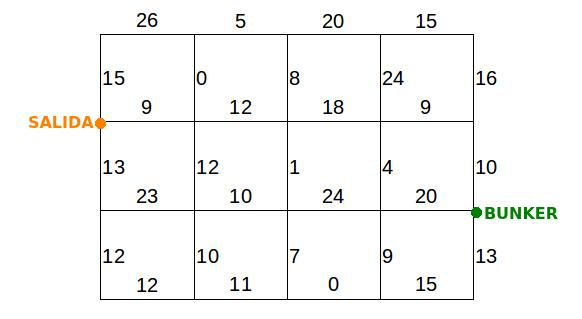
\includegraphics[scale=0.5]{imagenes/ejemplozombie.jpeg}
%	\end{center}
%	\caption{Ejemplo de ciudad para Zombieland II}\label{fig:ejzombie}
%\end{figure}
%
La solución para este ejemplo permite llegar al búnker sin perder ningún soldado, siendo el recorrido el indicado en la Figura \ref{fig:ejzombieres}.
%
%\begin{figure}[htb]
%	\begin{center}
%    		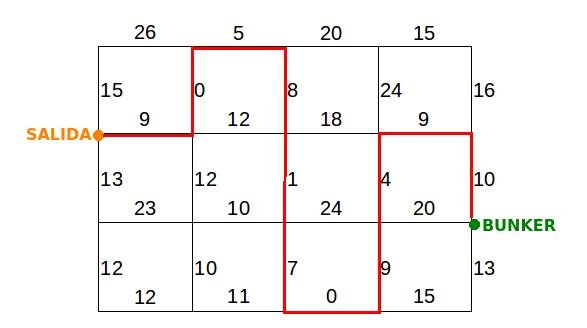
\includegraphics[scale=0.5]{imagenes/ejemplozombieres.jpeg}
%	\end{center}
%	\caption{Solución para el problema de la Figura \ref{fig:ejzombie}}\label{fig:ejzombieres}
%\end{figure}

\begin{figure}[!htb]
\minipage{0.5\textwidth}
  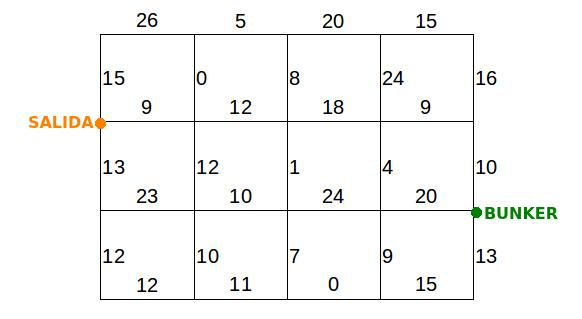
\includegraphics[scale=0.5]{imagenes/ejemplozombie.jpeg}
  \caption{Ejemplo de ciudad para Zombieland II}\label{fig:ejzombie}
\endminipage
\minipage{0.5\textwidth}
  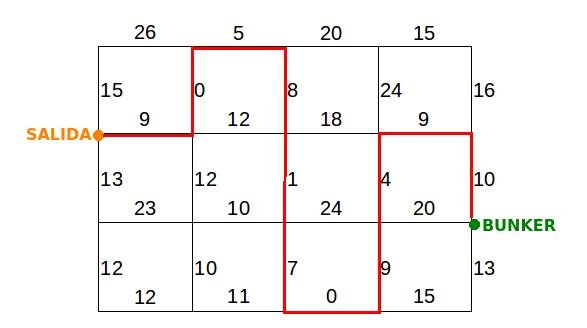
\includegraphics[scale=0.5]{imagenes/ejemplozombieres.jpeg}
  \caption{Solución para el problema de la Figura \ref{fig:ejzombie}}\label{fig:ejzombieres}
\endminipage
\end{figure}


\vspace*{0.6cm}

%\newpage
\subsection{Desarrollo de la idea y correctitud.}

\vspace*{0.3cm}

Llamemos $n$ la cantidad de calles horizontales y $m$ la cantidad de calles verticales.  Tomando $1 \leq i \leq n$ y $1 \leq j \leq m$, la esquina $(i,j)$ será la esquina formada por la intersección de las calles $i$ y $j$.  Para cada esquina definimos:

\begin{itemize}
	\item Dirigirse hacia {\bf arriba}: moverse a la esquina $(i-1,j)$. Esto no será válido cuando $i = 1$.
	\item Dirigirse hacia {\bf abajo}: moverse a la esquina $(i+1,j)$. Esto no será válido cuando $i = n$.
	\item Dirigirse hacia la {\bf izquierda}: moverse a la esquina $(i,j-1)$. Esto no será válido cuando $j = 1$.
	\item Dirigirse hacia la {\bf derecha}: moverse a la esquina $(i,j+1)$. Esto no será válido cuando $j = m$.
\end{itemize}

Debemos recorrer la ciudad en busca de un camino que permita llegar al búnker con la mayor cantidad de soldados vivos.  Sin embargo, probar todos los posibles caminos tomaría más tiempo del que disponemos.  Para optimizar esta búsqueda, hemos decidido buscar dicho camino de la siguiente manera:

Utilizando {\it backtraking}, encontrar las rutas que salen desde la posición de origen, de manera que ningún soldado muera.  Cada cuadra visitada será marcada para que ningún otro camino intente pasar por ahí, y así no tendremos caminos redundantes (es decir, no considerar distintos caminos que permitan llegar a una misma esquina con la misma cantidad de soldados vivos), y para cada esquina alcanzada se guardará la esquina anterior de ese camino y la cantidad de soldados vivos hasta ese momento.  Si en algún momento se llega a una esquina desde la cual no se puede avanzar sin pérdidas, vamos a señalizarla (en breve explicaremos para qué). 

Si por alguno de estos caminos se llega al búnker, entonces habremos encontrado una solución óptima.  Si ninguna de las rutas encontradas es solución, entonces deberemos animarnos a perder soldados.  Para ello, primero vamos a arriesgar sólo un soldado, es decir, si teníamos $s$ soldados iniciales, intentaremos llegar al búnker con $s-1$ soldados vivos. Entonces, retomaremos los caminos marcados anteriormente, a partir de las esquinas desde las que no podíamos avanzar sin pérdidas (reanunando cada una en el orden en el que fueron marcadas).  Desde ahí, avanzaremos armando los caminos que no nos produzcan más de una baja, y lo haremos de la misma manera que explicamos arriba: sin caminos redundantes y guardando la esquina antecesora y la cantidad de soldados vivos en cada esquina atravesada. 

Nuevamente, si alguno de estos caminos llega al búnker, será la solución.  Caso contrario repetiremos el procedimiento intentando llegar con $s-2$ soldados vivos. De forma sucesiva, nos animaremos a perder cada vez un soldado más, y el primer camino encontrado que llegue al búnker será retornado.  De esta manera, estamos asegurando que la solución tiene la mayor cantidad de soldados vivos al final.

Podría suceder que, durante el recorrido, se llegue a una esquina a partir de la cual cualquier camino elegido elimine la totalidad de soldados que se encuentran vivos hasta ese momento.  Esto quiere decir que, a partir de esa posición, no existe ningún camino posible hasta el búnker. Pero por como hemos diseñado el algoritmo, esa esquina quedaría marcada y cada vez que arriesguemos un soldado intentaremos avanzar inútilmente.  Para evitar estas vanas consultas, decidimos que en estos casos la esquina deje de ser considerada.

Veamos ahora que una misma esquina no puede ser visitada más de una cantidad $k$ fija de veces. En principio, cada esquina es incidida por hasta 4 cuadras.  Analicemos los siguientes casos:

\begin{itemize}
	\item Un camino llega a una esquina, y de ahí puede avanzar sin problemas por las otras 3 cuadras incidentes. En este caso, la esquina es visitada sólo una vez, ya que las 4 cuadras incidentes no vuelven a ser recorridas.
	\item Un camino llega a una esquina y de ahí puede avanzar por 2 de las 3 cuadras incidentes.  Si la cuadra restante elimina la totalidad de soldados, por lo dicho anteriormente, la esquina no vuelve a visitarse.  En caso contrario, la esquina queda marcada para reanudar el camino posteriormente pudiendo perder soldados. Puede suceder lo siguiente:
	\begin{itemize}
		\item Que al arriesgar soldados se pueda avanzar por esa cuadra, continuando el camino anterior. Entonces hay un sólo camino que visita esta esquina.
		\item Que un segundo camino pueda llegar a esta esquina a través de la cuadra restante.  En este caso, hay 2 visitas a la esquina, pero la segunda no podrá seguir avanzando, puesto que las otras 3 cuadras ya fueron recorridas.  Se tienen entonces 2 visitas a la esquina pero sólo nos interesa el primer camino, por lo cual no guardaremos los datos del segundo.
	\end{itemize}
	\item %Un camino llega a una esquina y de ahí puede avanzar por 1 de las 3 cuadras incidentes.  Si alguna de las cuadras restantes elimina
\end{itemize}

\vspace*{0.6cm}

%\newpage
%\subsection{Justificación de la resolución y demostración de correctitud.}

%\vspace*{0.3cm}



%\vspace*{0.6cm}

%\newpage
\subsection{Análisis de complejidad.}

\vspace*{0.3cm}


\vspace*{0.6cm}

%\newpage
\subsection{Experimentación y gráficos.}


\subsubsection{Test 1}

\vspace*{0.3cm}


\vspace*{0.6cm}

%\newpage
\subsubsection{Test 2}


\newpage